\documentclass[letterpaper,11pt]{article}
\usepackage{fullpage}
\usepackage{graphicx}
\usepackage{underscore}
\usepackage{siunitx}

\newcommand{\net}[1]{\textsf{#1}}
\newcommand{\Net}[1]{\ensuremath{\overline{\textsf{#1}}}}
\newcommand{\Wbar}{\ensuremath{\overline{\textsf{W}}}}
\newcommand{\Vcc}{\net{Vcc}}
\newcommand{\GND}{\net{GND}}
\newcommand{\Pin}[1]{\textbf{Pin #1}}
\newcommand{\pin}[1]{\textbf{pin #1}}
\newcommand{\pins}[1]{\textbf{pins #1}}
\newcommand{\npin}[2]{\pin{#1} (\net{#2})}
\newcommand{\Npin}[2]{\pin{#1} (\Net{#2})}
\newcommand{\rpin}[2]{\refdes{#1} \pin{#2}}
\newcommand{\rpins}[2]{\refdes{#1} \pins{#2}}
\newcommand{\rnpin}[3]{\refdes{#1} \pin{#2} (\net{#3})}
\newcommand{\rNpin}[3]{\refdes{#1} \pin{#2} (\Net{#3})}
\newcommand{\rnpins}[3]{\refdes{#1} \pins{#2} (\net{#3})}
\newcommand{\refdes}[1]{\textbf{#1}}
\newcommand{\kohm}[1]{\SI{#1}{\kilo\ohm}}
\newcommand{\Mohm}[1]{\SI{#1}{\mega\ohm}}
\newcommand{\pF}[1]{\SI{#1}{\pico\farad}}
\newcommand{\uF}[1]{\SI{#1}{\micro\farad}}
\newcommand{\V}[1]{\SI{#1}{\volt}}
\newcommand{\MHz}[1]{\SI{#1}{\mega\hertz}}
\title{Ultim809 Rev 0 Board Bringup Procedure}
\author{Matt Sarnoff}
\date{\today}

\begin{document}
\maketitle
\section{Board Errors}
\subsection{\refdes{U4} \net{TSC}}
\Pin{39} of \refdes{U4} (\net{TSC}) is incorrectly connected to \Vcc. It should be connected to \GND. Cut the trace on the top side of the board as follows:

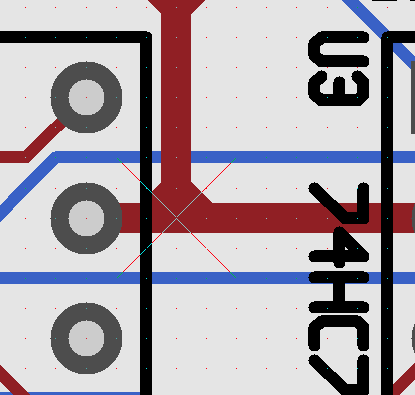
\includegraphics[width=2in]{badtrace1a.png}
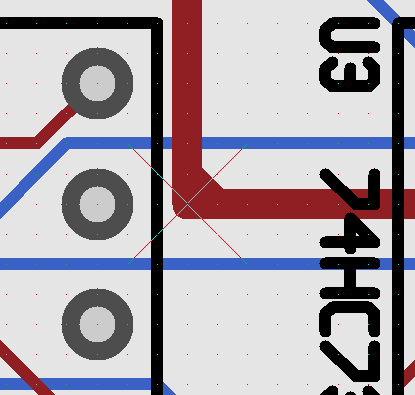
\includegraphics[width=2in]{badtrace1b.png}

On the bottom of the board, solder a piece of enameled magnet wire or wire-wrap wire from \pin{39} to \pin{1}.

\subsection{\refdes{U16} \net{TX} and \net{RX} swapped}
\rnpin{U16}{10}{RX} is mistakenly connected to \rnpin{J2}{5}{RXD}, and \rnpin{U16}{11}{TX} is mistakenly connected to \rnpin{J2}{4}{TXD}. These two need to be swapped. Since it is difficult to fix this on the board, you will have to fashion an adapter on a piece of perfboard.

\subsection{\Net{CSW} and \Net{CSR} swapped}
\rNpin{U21}{14}{CSW} is mistakenly connected to \rpin{U17}{11} and \rNpin{U21}{15}{CSR} is mistakenly connected to \rpin{U17}{10}. The two should be swapped. Cut traces on the back of the board at \rpin{U17}{10-11}. Add a wire from \rpin{U17}{11} to \rpin{U21}{15} and a wire from \rpin{U17}{10} to \rpin{U21}{14}.

\subsection{VRAM bus incorrect}
Cut the traces on the back of the board at \rpin{U23}{12} and \rpin{U26}{26}. Add a wire from \rpin{U23}{19} to \rpin{U26}{4} and a wire from \rpin{U24}{19} to \rpin{U26}{26}.

\section{Assembly and testing}

\subsection{Sockets}
\begin{itemize}
\item Install all IC sockets.
\end{itemize}

\subsection{Power}
\begin{itemize}
\item Install \refdes{D2} (power LED), \refdes{R3} (\kohm{1}), \refdes{D1} (1N4001), \refdes{C2} and \refdes{C4} (\uF{0.1}), \refdes{C1} and \refdes{C3} (\uF{10} electrolytic, rated for \V{50}), \refdes{U1} (7805), \refdes{J1}, and \refdes{S1}.
\item Ensure \refdes{S1} is in the down (disconnected) position.
\item Connect \V{9} DC power to \refdes{J1}. The center pin is positive and the outer ring is ground.
\item Turn on \refdes{S1}. \refdes{D2} should light.
\item Measure \Vcc\ (for example, at \refdes{U14} \pin{16}) and ensure it is roughly \V{5}.
\end{itemize}

\subsection{Clock signals}
\begin{itemize}
\item Install \refdes{X1} (\MHz{8}), \refdes{U3} (74HC73), and decoupling capacitor \refdes{C16}.
\item Turn on power.
\item Using a frequency counter, measure the clock signals. \rpin{U3}{1} should read \MHz{8}. \rnpin{U4}{34}{E} and \rnpin{U4}{35}{Q} should read \MHz{2}.
\item Using a two-channel oscilloscope or logic analyzer, observe the \net{E} (\rpin{U4}{34}) and \net{Q} (\rpin{U4}{35}) waveforms.

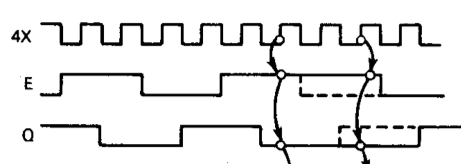
\includegraphics[width=4in]{clockwaves.png}
\end{itemize}

\subsection{Processor integrity}
\begin{itemize}
\item Install \refdes{RN1} (\kohm{10}), \refdes{C6} (\uF{10}), \refdes{D3} and \refdes{D4}, \refdes{R4} and \refdes{R5} (\kohm{1}), \refdes{S5}, \refdes{S2}, and \refdes{S3}.
\item Flip \refdes{S5} up to HALT.
\item Turn on power.
\item Ensure \rNpin{U4}{40}{HALT} is \V{0}.
\item Ensure \Npin{U4}{37}{RESET}, \Npin{2}{NMI}, \Npin{3}{IRQ}, and \Npin{4}{FIRQ} are \V{5}.
\item Flip \refdes{S5} down to RUN and ensure \pin{40} is \V{5}.
\item Ensure \pin{37} is \V{0} when \refdes{S2} is depressed and \pin{2} is \V{0} when \refdes{S3} is depressed.
\item Turn off power, install \refdes{U4} (68B09E) and decoupling capacitor \refdes{C17}.
\item Flip \refdes{S5} up to HALT and turn on power.
\item Ensure \refdes{D3} and \refdes{D4} are both lit. This indicates the processor is in good condition.
\end{itemize}

\subsection{ROM, program execution, and address decoding}
\begin{itemize}
\item Burn \texttt{romtest1.s19} to an 8K$\times$8 EEPROM, using the Arduino ROMBurner and the \texttt{ser09} utility.
\item Install the EEPROM in \refdes{U9}, and install \refdes{U5} (74HC00), \refdes{U7} (74HC139), \refdes{RN3} (\kohm{10}), \refdes{S4}, and associated decoupling capacitors.
\item Flip \refdes{S4} to the left (EEPROM WRITE PROTECT ON) and ensure \rNpin{U9}{27}{WE} is connected to \rpin{RN3}{6}. (Resistance between \pin{27} and \Vcc\ is \kohm{10}.)
\item Flip \refdes{S4} to the right (EEPROM WRITE PROTECT OFF) and ensure \pin{27} is connected to \rNpin{U8}{29}{WR}.
\item Flip \refdes{S4} to the left and flip \refdes{S5} to HALT.
\item Turn on power. \refdes{D3} and \refdes{D4} should light.
\item Flip \refdes{S5} to RUN. \refdes{D3} and \refdes{D4} should turn off. The program should now be running. After about one second, \refdes{D3} should light (SYNC acknowledge), indicating the test program is finished. Pressing \refdes{S2} or \refdes{S3} will restart the program: the light will go out, and should come on about a second later.
\item Turn off power.
\item With a logic analyzer, attach probes to \rnpins{U4}{8-23}{A0-A15}, \rnpin{U4}{34}{E}, \rnpin{U4}{32}{R/\Wbar}, \rNpin{U5}{6}{RAMSEL}, \rNpin{U7}{4}{IOSEL}, \rNpin{U7}{5}{ROMSEL}, \rNpin{U7}{9}{RD}, and \rNpin{U7}{10}{WR}. The positive edge of \net{E} should be used as the clock signal.
\item Set \refdes{S5} to HALT, run the logic analyzer, and set \refdes{S5} to RUN. Repeat multiple times to verify the following truth table:

\begin{minipage}[t]{0.3\textwidth}
\begin{tabular}[t]{|c|c|c|c|}
\hline
\net{E} & \net{R/\Wbar} & \Net{RD} & \Net{WR} \\
\hline\hline
0 & x & 1 & 1 \\
1 & 1 & 0 & 1 \\
1 & 0 & 1 & 0 \\
\hline
\end{tabular}
\end{minipage}
\begin{minipage}[t]{0.5\textwidth}
\begin{tabular}[t]{|c|c|c|c|}
\hline
\net{A0-A15} & \Net{RAMSEL} & \Net{IOSEL} & \Net{ROMSEL} \\
\hline\hline
\$0xxx & 0 & 1 & 1 \\
\$1xxx & 0 & 1 & 1 \\
\$2xxx & 0 & 1 & 1 \\
\$3xxx & 0 & 1 & 1 \\
\$4xxx & 0 & 1 & 1 \\
\$5xxx & 0 & 1 & 1 \\
\$6xxx & 0 & 1 & 1 \\
\$7xxx & 0 & 1 & 1 \\
\$8xxx & 0 & 1 & 1 \\
\$9xxx & 0 & 1 & 1 \\
\$Axxx & 0 & 1 & 1 \\
\$Bxxx & 0 & 1 & 1 \\
\hline
\$Cxxx & 1 & 0 & 1 \\
\$Dxxx & 1 & 0 & 1 \\
\hline
\$Exxx & 1 & 1 & 0 \\
\$Fxxx & 1 & 1 & 0 \\
\hline
\end{tabular}
\end{minipage}

The test program attempts to read and write to successive addresses, so the address decoding may be observed.
\end{itemize}

\subsection{I/O decoding}
\begin{itemize}
\item Install \refdes{U6} (74HC14), \refdes{U10} (74HC138), and associated decoupling capacitors.
\item Attach logic analyzer probes to \rnpins{U4}{8-23}{A0-A15}, \rNpin{U10}{15}{VIASEL}, \rNpin{U10}{14}{UARTSEL}, \rNpin{U10}{13}{SRSEL}, \rNpin{U10}{12}{AVSEL}, \rNpin{U10}{11}{EXT1SEL}, \rNpin{U10}{10}{EXT2SEL}, \rNpin{U10}{9}{EXT3SEL}, \rNpin{U10}{7}{EXT4SEL}, and \rNpin{U5}{8}{EXTIOSEL}. The positive edge of \net{E} should be used as the clock signal.
\item Run \texttt{romtest1.s19} again and verify the following truth table: 

\begin{tabular}[t]{|c|c|c|c|c|c|c|c|c|c|}
\hline
\net{A0-A15} & \Net{VIA} & \Net{UART} & \Net{SR} & \Net{AV} & \Net{EXT1} & \Net{EXT2} & \Net{EXT3} & \Net{EXT4} & \Net{EXTIO} \\
\hline\hline
\$Bxxx & 1 & 1 & 1 & 1 & 1 & 1 & 1 & 1 & 1 \\
\$C000-\$C3FF & 0 & 1 & 1 & 1 & 1 & 1 & 1 & 1 & 1 \\
\$C400-\$C7FF & 1 & 0 & 1 & 1 & 1 & 1 & 1 & 1 & 1 \\
\$C800-\$CBFF & 1 & 1 & 0 & 1 & 1 & 1 & 1 & 1 & 1 \\
\$CC00-\$CFFF & 1 & 1 & 1 & 0 & 1 & 1 & 1 & 1 & 1 \\
\$D000-\$D3FF & 1 & 1 & 1 & 1 & 0 & 1 & 1 & 1 & 0 \\
\$D400-\$D7FF & 1 & 1 & 1 & 1 & 1 & 0 & 1 & 1 & 0 \\
\$D800-\$DBFF & 1 & 1 & 1 & 1 & 1 & 1 & 0 & 1 & 0 \\
\$DC00-\$DFFF & 1 & 1 & 1 & 1 & 1 & 1 & 1 & 0 & 0 \\
\$Exxx & 1 & 1 & 1 & 1 & 1 & 1 & 1 & 1 & 1 \\
\hline
\end{tabular}
\end{itemize}

\subsection{UART}
\begin{itemize}
\item Install \refdes{U16} (16C550), decoupling capacitor \refdes{C29}, \refdes{R10} (\Mohm{1}), \refdes{R11} (\kohm{1.5}), \refdes{C8} (\pF{27}), \refdes{C9} (\pF{47}), \refdes{X2} (\MHz{1.8432}), \refdes{J2}, \refdes{R1} (\SI{330}{\ohm}), \refdes{R2} (\kohm{1.5}), and \refdes{D5}. Orient \refdes{D5} so the shortest lead (the green anode) is on the left and is inserted into the square hole.
\item Burn \texttt{romtest2.s19} onto the EEPROM.
\item Connect a \V{5} FTDI USB-to-serial cable to \refdes{J2}, with the black wire on the right. Connect the other end to a PC. Start a terminal program listening at 38400 baud, 8 data bits, no parity, 1 stop bit.
\item Turn on the system and run the program.
\item The status LED \refdes{D5} should turn off and the system should print the following:
\begin{verbatim}
Hello World!
Type r, y, g, or o to change LED color
\end{verbatim}
Typing one of the four letters from the terminal changes the LED color (red, yellow, green, off) and prints a message. (``\texttt{Red.}'' or ``\texttt{Yellow.}'' or ``\texttt{Green.}'' or ``\texttt{Off.}'')
\item Additionally, use a frequency counter to check the UART's clock rate at \rpin{U16}{9}. It should be $16\times$ the baud rate: in this case, approximately \SI{614400}{\hertz}.
\end{itemize}

\subsection{RAM and bank switching}
\begin{itemize}
\item Install diode \refdes{D7} (1N4148).
\item Test \refdes{D7} using a multimeter in diode mode. Place the positive lead on \rNpin{U4}{4}{FIRQ} and place the negative lead on \rNpin{U11}{21}{IRQ}. (\refdes{U11} should not be installed yet.) The meter should read a small positive voltage. Reverse the leads and the meter should indicate an open circuit.
\item Install \refdes{U8} (512K SRAM), \refdes{U11} (W65C22S), \refdes{U12} (74HC157), \refdes{U13} (74HC08), and associated decoupling capacitors.
\item Burn \texttt{romtest3.s19} onto the EEPROM.
\item Connect the serial cable and start the terminal as in the previous step.
\item Run the program. It tries to determine the size of the RAM by cycling through the 16K pages and counting them until it detects wraparound. It should print
\begin{verbatim}
0512KB RAM available.
\end{verbatim}
on the console.
\end{itemize}

\subsection{Audio/video I/O decoding}
\begin{itemize}
\item Install \refdes{U17} (74HC139), \refdes{U18} (74HC02), \refdes{U19} (74HC74), and associated decoupling capacitors.
\item Burn \texttt{romtest4.s19} onto the EEPROM.
\item Attach logic analyzer probes to \rNpin{U17}{1}{AVSEL}, \rnpin{U17}{2-3}{A1-A2}, \rNpin{U17}{4}{VDPSEL}, \rNpin{U17}{5}{PSGSEL}, \rNpin{U17}{6}{FF1SEL}, \rNpin{U17}{7}{FF2SEL}, \rNpin{U17}{13}{RD}, \rNpin{U17}{14}{WR}, \rNpin{U17}{10}{CSR}, \rNpin{U17}{11}{CSW}, \rnpin{U18}{3}{A0}, \rnpin{U18}{1}{BC1}, \rnpin{U18}{4}{BDIR}, \rnpin{U18}{13}{FF1CP}, \rnpin{U18}{10}{FF2CP}, \rnpin{U19}{3}{A3}, \rnpin{U19}{5}{VBANK}, and \rnpin{U19}{9}{PADSELECT}. The positive edge of \net{E} should be used as the clock signal.
\item Run the program and verify the following truth tables:

\begin{tabular}{|c|c|c|c|c|c|c|c|c|c|}
\hline
\Net{AVSEL} & \net{A0-A2} & \Net{RD} & \Net{WR} & \Net{VDPSEL} & \Net{PSGSEL} & \Net{FF1SEL} & \Net{FF2SEL} & \Net{CSR} & \Net{CSW} \\
\hline
1 & \%xxx & x & x &   1 & 1 & 1 & 1 &   1 & 1 \\
0 & \%00x & 1 & 0 &   0 & 1 & 1 & 1 &   1 & 0 \\
0 & \%00x & 0 & 1 &   0 & 1 & 1 & 1 &   0 & 1 \\
0 & \%01x & x & x &   1 & 0 & 1 & 1 &   1 & 1 \\
0 & \%10x & x & x &   1 & 1 & 0 & 1 &   1 & 1 \\
0 & \%11x & x & x &   1 & 1 & 1 & 0 &   1 & 1 \\
\hline
\end{tabular}

\begin{tabular}{|c|c|c|c|c|c|c|}
\hline
\Net{AVSEL} & \Net{PSGSEL} & \net{A0-A2} & \Net{RD} & \Net{WR} & \net{BC1} & \net{BDIR} \\
\hline
1 & 1 & \%xxx & x & x & 0 & 0 \\
0 & 0 & \%010 & x & 0 & 1 & 1 \\
0 & 0 & \%010 & x & 1 & 1 & 0 \\
0 & 0 & \%011 & x & 0 & 0 & 1 \\
0 & 0 & \%011 & x & 1 & 0 & 0 \\
\hline
\end{tabular}

\begin{tabular}{|c|c|c|c|c|c|c|c|c|}
\hline
\Net{AVSEL} & \Net{FF1SEL} & \Net{FF2SEL} & \Net{RD} & \net{A3} & \net{FF1CP} & \net{FF2CP} & \net{VBANK} & \net{PADSELECT} \\
\hline
1 & 1 & 1 &   x & x &  0 & 0 &  no change & no change \\
0 & 0 & 1 &   1 & x &  0 & 0 &  no change & no change \\
0 & 0 & 1 &   0 & 0 &  1 & 0 &  0 & no change \\
0 & 0 & 1 &   0 & 1 &  1 & 0 &  1 & no change \\
0 & 1 & 0 &   0 & 0 &  0 & 1 &  no change & 0 \\
0 & 1 & 0 &   0 & 1 &  0 & 1 &  no change & 1 \\
\hline
\end{tabular}
\end{itemize}

\subsection{Audio/gamepads}
\begin{itemize}
\item Install \refdes{U20} (YM2149), \refdes{R6}, \refdes{R7}, and \refdes{R8} (\kohm{1}), \refdes{R9} (\kohm{4.7}), \refdes{C7} (\uF{1}), \refdes{J9}, and \refdes{J10}. Also install decoupling capacitors.
\end{itemize}

\subsection{Video}
\begin{itemize}
\item Install \refdes{U21} (TMS9918A), \refdes{U22} (74HC04), \refdes{U23}, \refdes{U24}, and \refdes{U25} (74HC574), \refdes{U26} (62256), \refdes{D6} (1N4148), \refdes{C10} and \refdes{C11} (\pF{33}), \refdes{X3} (\MHz{10.738635}), \refdes{R19} (\SI{470}{\ohm}), \refdes{R20} and \refdes{R21} (\SI{75}{\ohm}), \refdes{C12} (\uF{22}), \refdes{C13} (\uF{0.1}), \refdes{C15} (\uF{220}), \refdes{L1} (ferrite bead), \refdes{Q1} (2N3904), and \refdes{J6}. Also install decoupling capacitors.
\end{itemize}

\end{document}